\subsection{Ensamblaje Final}

\par \noindent
Para realizar el ensamblaje final del dispositivos debió imprimir los moldes previamente diseñados. La impresora 3D que se utilizó para la impresión del diseño tridimensional es la de la figura 2.22. El resultado de las impresiones son las siguientes:

\begin{figure}[H]
	\centering
	\includegraphics[width=\linewidth]{ensamblaje01.png}
	\caption{Impresora 3D en el proceso de impresión del armazón}
\end{figure}

\begin{figure}[H]
	\centering
	\includegraphics[width=\linewidth]{ensamblaje02.png}
	\caption{Armazón del prototipo hecho por una impresora 3D}
\end{figure}

\par \noindent
El armazón una vez impreso se inicia a soldar los componentes en la placa o circuito impreso del prototipo.

\begin{figure}[H]
	\centering
	\includegraphics[width=\linewidth]{ensamblaje03.png}
	\caption{Circuito Impreso Antes y Despues de soldar sus componentes}
\end{figure}

\par \noindent
Por ultimo queda colocar la bateria y su circuito en el molde inferior, luego a la placa del dispositivo, después la pantalla LCD y al final colocamos el molde superior.

\begin{figure}[H]
	\centering
	\includegraphics[width=0.8\linewidth]{ensamblaje04.png}
	\caption{Proceso del ensamblaje del prototipo de medición de temperatura}
\end{figure}

\par \noindent
El resultado de unir todas las piezas sería el siguiente:

\begin{figure}[H]
	\centering
	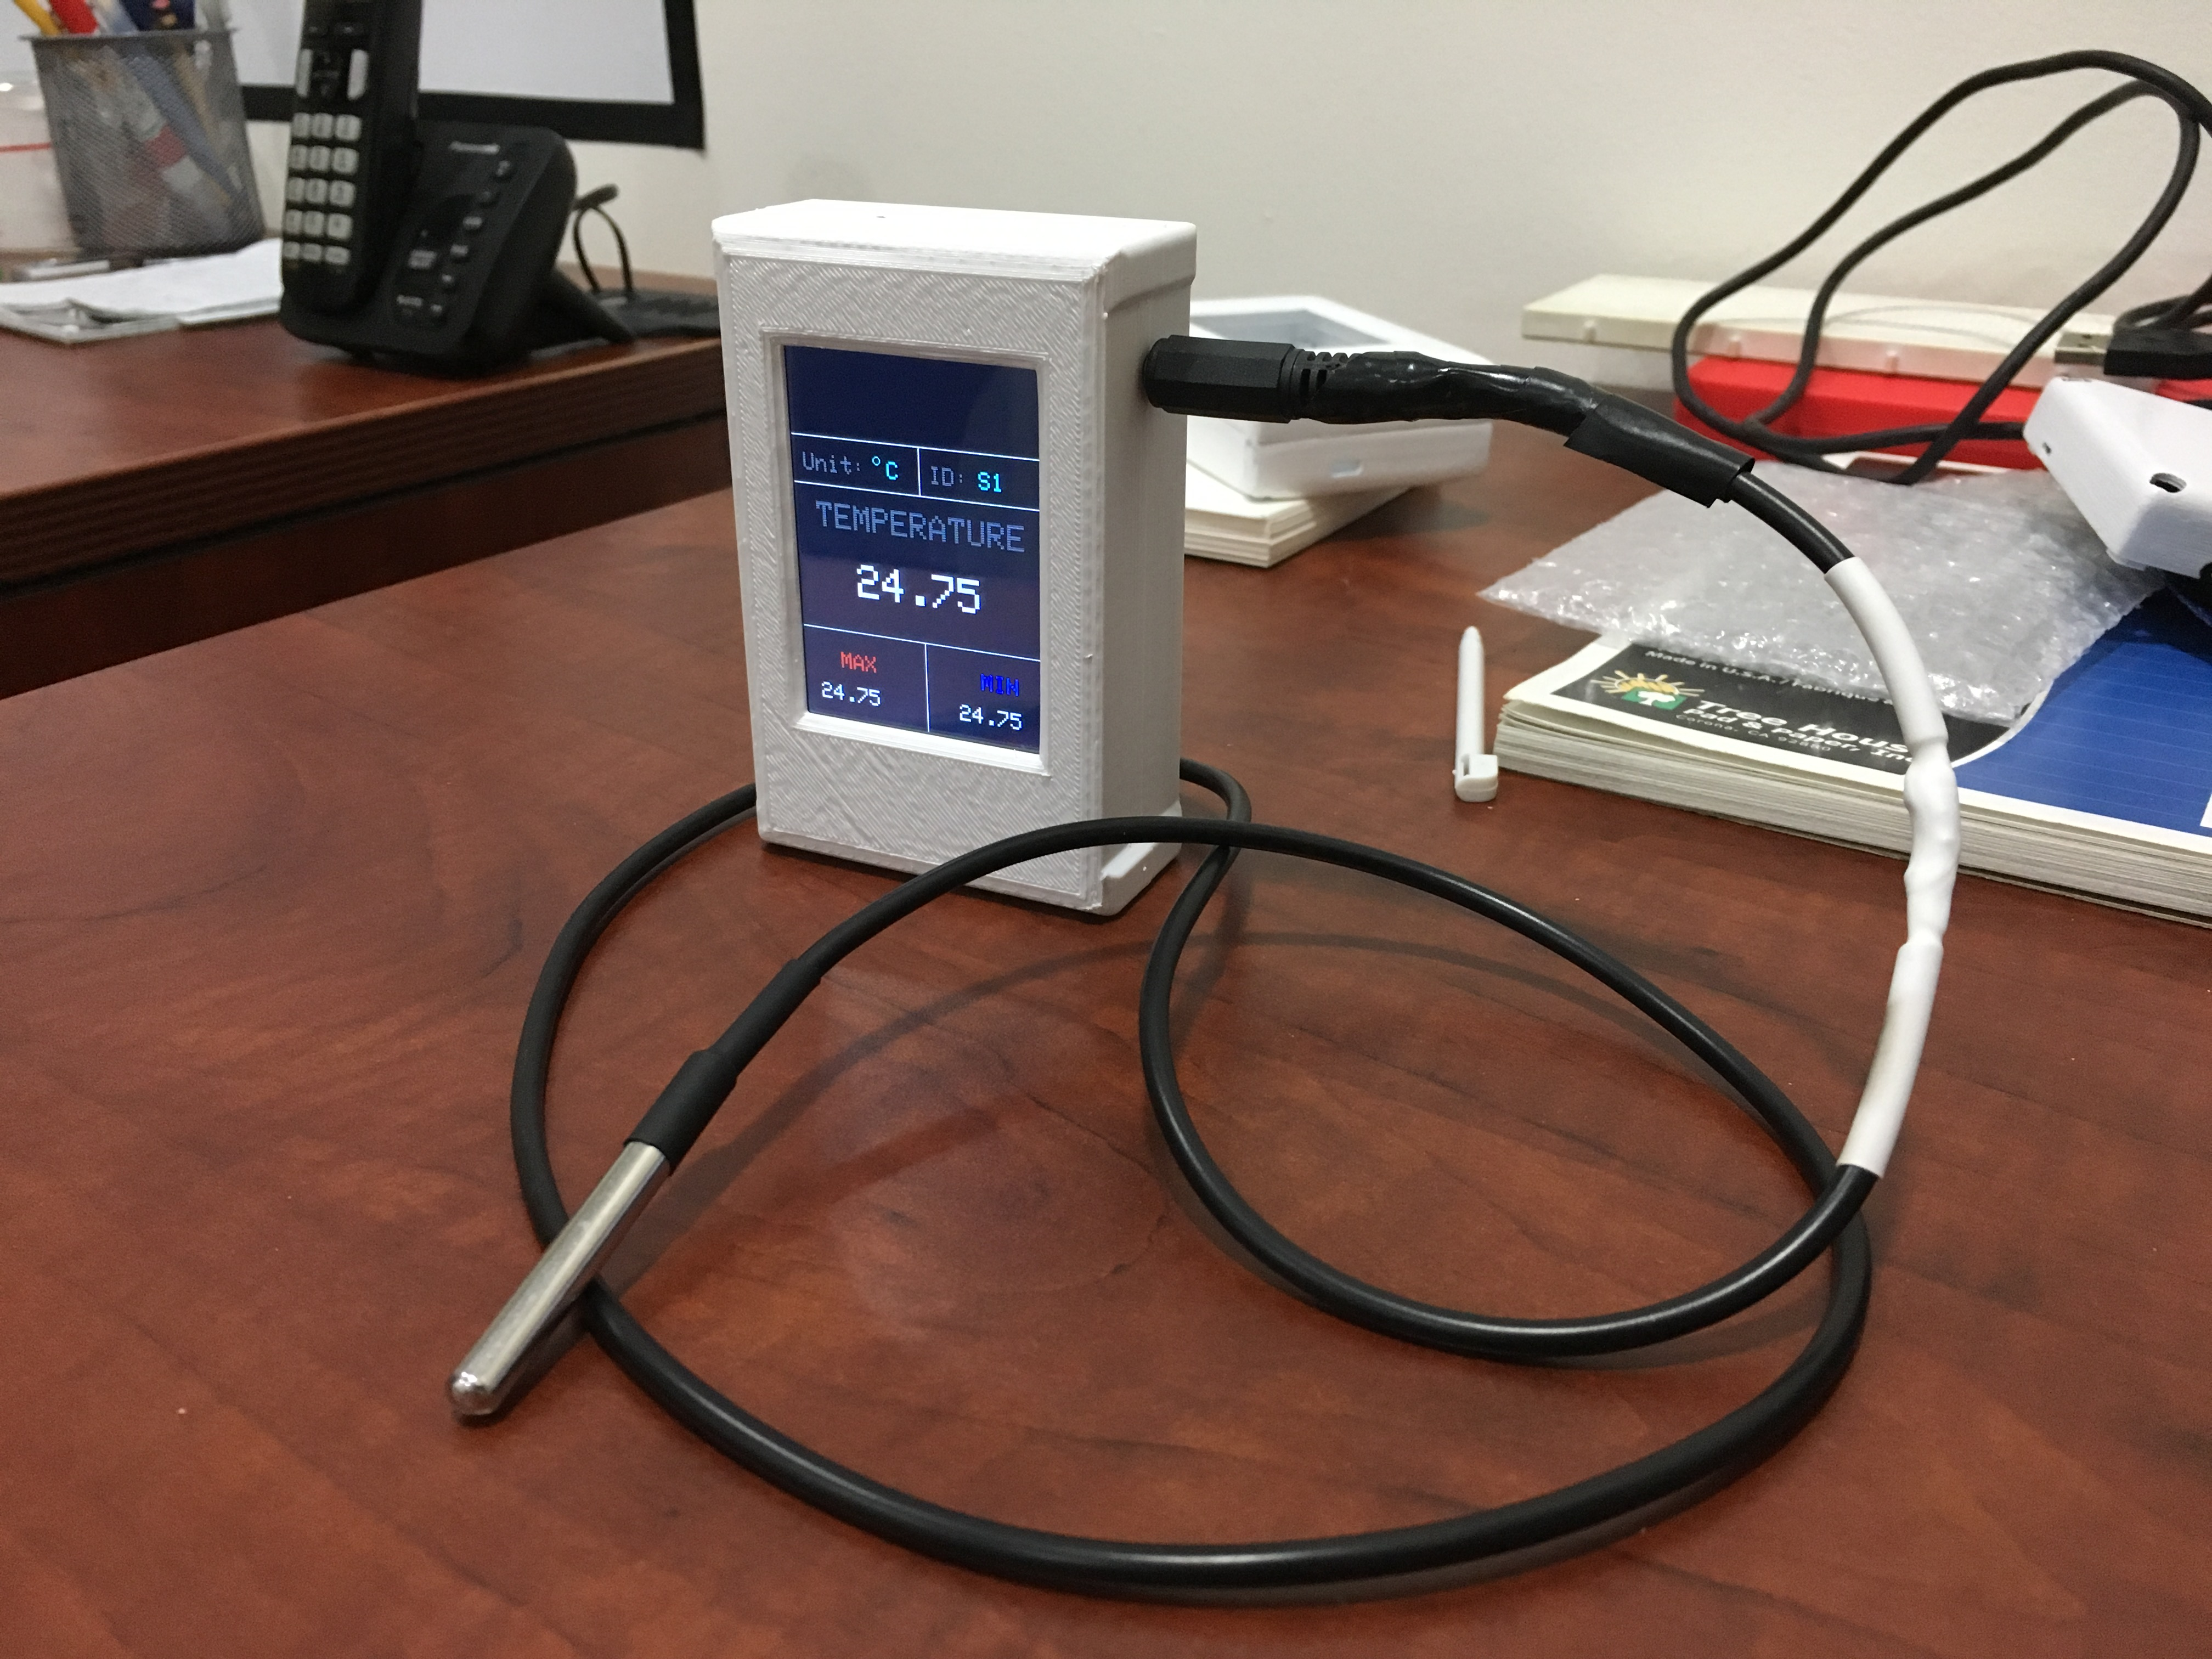
\includegraphics[width=0.8\linewidth]{ensamblaje05.jpg}
	\caption{Prototipo de medición de temperatura completo en su versión 1.0}
\end{figure}

\par \noindent
Ahora que se terminó la elaboración del prototipo deseado, se tomo en cuenta al momento de seleccionar los componentes elegimos el sensor de temperatura DS18B20 por su margen de error y su bajo costo. Ahora la preguntas son las siguientes: ¿El prototipo cumple con los estadares de la compañia SIGCSA? y ¿Cuánto es el costo de la elaboración de un prototipo de estos? para ellos hicierón análisis de las mediciones de temperatura para establecer conclusiones en la sección de resultados.